\chapter{Arhitektura i dizajn sustava}
		
		Arhitektura se može podijeliti na tri glavna dijela:
		
		\begin{itemize}
			\item 	\textit{REST API poslužitelj (Spring Boot)}
			\item 	\textit{Klijentska aplikacija (React)}
			\item 	\textit{Baza podataka}		
		\end{itemize}
		
		\begin{figure}[h]
			\centering
			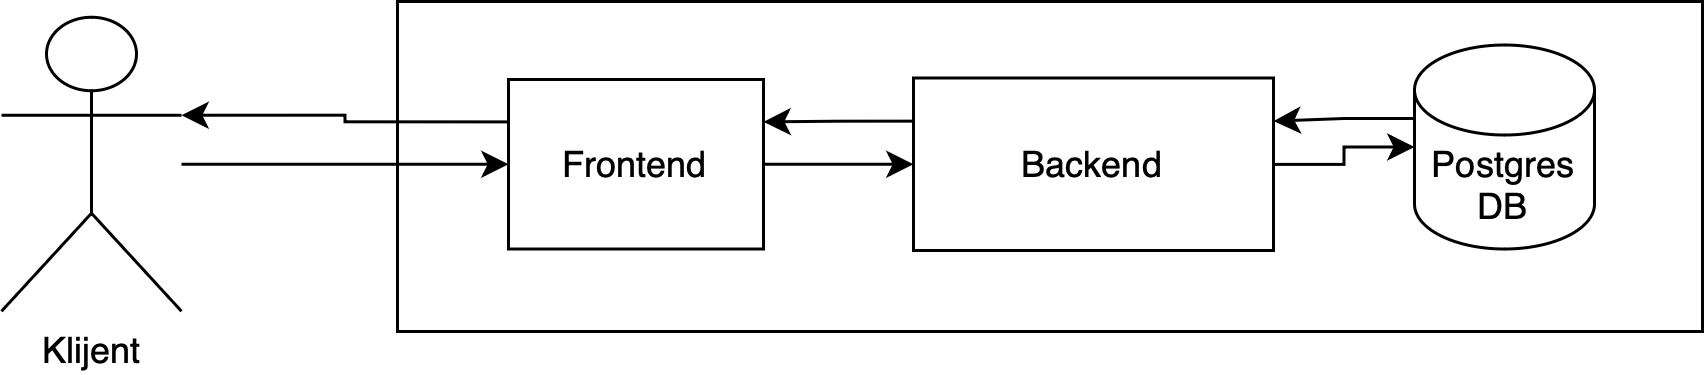
\includegraphics[width=0.8\linewidth]{./slike/arhitektura_sustava.png} 
			\caption{Arhitektura sustava}
			\label{fig:arh_sustava}
		\end{figure}
		
		
		
		Korisnik interagira s klijentskom aplikacijom putem web preglednika. Ova aplikacija je odvojena od backend sustava te koristi React uz typescript za stvaranje dinamičkog korisničkog sučelja.
		
		REST API poslužitelj izgrađen je koristeći Spring Boot, koji omogućuje izradu visoko efikasnih i skalabilnih RESTful servisa. Komunikacija između klijenta i servera odvija se putem HTTP protokola, gdje frontend šalje zahtjeve backendu, a backend odgovara s potrebnim podacima u JSON formatu.
		
		Klijentska aplikacija je odgovorna za prikazivanje podataka korisniku i obradu korisničkih interakcija. Ona komunicira s backendom putem REST API-ja za dohvaćanje i slanje podataka.
		
		Postgres baza podataka čuva sve podatke potrebne za aplikaciju. Spring Boot aplikacija komunicira s bazom podataka koristeći Spring Data JPA za upravljanje podacima.
		
		Odlučili smo se za korištenje Intellij-a kao razvojnog okruženja za backend, a za frontend koristimo Visual Studio Code.
		Za razliku od tradicionalnog MVC koncepta, naš sustav je podijeljen na odvojene slojeve gdje backend (REST API poslužitelj) i frontend (klijentska aplikacija) rade neovisno jedan o drugome. Uspoređujući s tradicionalnim MVC konceptom, mogli bismo reći da je View (V u MVC) na frontendu, a Model I Controller (M I C u MVC) na backendu. Ovo omogućuje fleksibilnost i lakše skaliranje svakog dijela aplikacije zasebno.
				

				
		\section{Baza podataka}

			Za potrebe naše aplikacije korisiti ćemo relacijsku bazu podataka kako bismo lakše oblikovali stvarni svijet. Baza nam je potrbna za metodičku pohranu podataka te njihovo brzo dohvaćanje. Naša baza podataka se sastoji od sljedećih entiteta:
			
			\begin{packed_item}
				\item Patient
				\item Accommodation
				\item AccommodationOrder
				\item AccommodationBooking
				\item TransportCompany
				\item TransportVehicle
				\item TransportBooking
				\item MedicalAppointment
				\item AdminRole
				\item AdminRoles
				\item Admin
			\end{packed_item}
		
			\subsection{Opis tablica}
			
				
				\noindent
				\textbf{Patient} Ovaj entitet sadrži sve informacije o korisniku usluga našeg sustava. Kako su svi korisnici pacijenti odlučili smo ih imenovati tako. Entitet sadrži atribute: patient\_ID, first\_name, last\_name, PIN, email i phone\_number. Ovaj entitet je u vezi \textit{One-to-Many} s entitetom AccommodationOrder preko atributa patient\_ID.
				
				\begin{longtblr}[
					label=none,
					entry=none
					]{
						width = \textwidth,
						colspec={|X[6,l]|X[6, l]|X[20, l]|}, 
						rowhead = 1,
					} %definicija širine tablice, širine stupaca, poravnanje i broja redaka naslova tablice
				
					\hline 
					\SetCell[c=3]{c}{\textbf{Patient}}\\
					\hline[3pt]
					\SetCell{LightGreen}patient\_ID & VARCHAR & primarni ključ tablice \\
					\hline
					first\_name	& VARCHAR &  ime pacijenta\\ 
					\hline 
					last\_name & VARCHAR &  prezime pacijenta \\ 
					\hline 
					PIN & VARCHAR	&  Personal Identification Number, kao OIB u hrvatskoj\\ 
					\hline 
					email & VARCHAR & pacijentov email\\ 
					\hline	
					phone\_number & VARCHAR & pacijentov telefonski broj \\
					\hline
				\end{longtblr}
			
				\noindent
				\textbf{Accommodation} Ovaj entitet sadržava potrebne podatke o nekom smještaju koji je smještajni administrator unio. Entitet sadrži atribute: accommodation\_ID, type, address, availibility\_start, availability\_end i location. Ovaj entitet je u \textit{One-to-Many} vezi s entitetom AccommodationBooking preko atributa accommodation\_ID.
				
				\begin{longtblr}[
					label=none,
					entry=none
					]{
						width = \textwidth,
						colspec={|X[10,l]|X[6, l]|X[18, l]|}, 
						rowhead = 1,
					} %definicija širine tablice, širine stupaca, poravnanje i broja redaka naslova tablice
					\hline 
					\SetCell[c=3]{c}{\textbf{Accommodation}}\\ 
					\hline[3pt]
					\SetCell{LightGreen}accommodation\_ID & VARCHAR & primarni ključ tablice\\ 
					\hline
					type & VARCHAR & vrsta smještaja \\
					\hline 
					address & VARCHAR & adresa smještaja \\
					\hline
					availability\_start & DATETIME & datum i vrijeme od kada je smještaj dostupan \\
					\hline
					availability\_end & DATETIME & datum i vrijeme do kada je smještaj dosupan \\
					\hline
					location & POINT & kordinate smještaja \\
					\hline
				\end{longtblr}
			
			\noindent
			\textbf{AccommodationOrder} Ovaj entitet se koristi za pohravnjivanje pacijentovih zahtjeva o traženom smještaju. U slučaju da traženi smještaj nije odmah dostupan zahtjev se sprema kako bih se kasnije mogao opet pogledati. Entitet sadrži atribute: accommodation\_order\_ID, arrival\_datetime, departure\_datetime, accommodation\_type i patient\_ID. Ovaj entitet je u \textit{Many-to-One} vezi s entitetom Patient preko atributa patient\_id i u vezi \textit{One-to-One} s entitetom AccommodationBooking preko atributa accommodation\_booking\_id.
			\begin{longtblr}[
				label=none,
				entry=none
				]{
					width = \textwidth,
					colspec={|X[15,l]|X[6, l]|X[20, l]|}, 
					rowhead = 1,
				} %definicija širine tablice, širine stupaca, poravnanje i broja redaka naslova tablice
				\hline 
				\SetCell[c=3]{c}{\textbf{AccommodationOrder}}\\ 
				\hline[3pt]
				\SetCell{LightGreen}accommodation\_order\_ID & VARCHAR & primarni ključ tablice\\ 
				\hline
				arrival\_datetime & DATETIME & vrijeme dolaska pacijenta u državu, od tada mu treba smještaj\\
				\hline
				departure\_datetime & DATETIME & vrijeme odlaska pacijenta iz države, do tada treba smještaj \\
				\hline
				accommodation\_type & VARCHAR & željeni tip smještaja koji pacijent traži \\
				\hline
				location & VARCHAR & kordinate područja na kojem je potrebno naći smještaj \\
				\hline
				\SetCell{LightBlue} patient\_ID	& VARCHAR & ID pacijenta koji je napravio ovaj zahtjev \\
				\hline 
				\SetCell{LightBlue} accommodation\_booking\_id	& VARCHAR & ID bookinga koji je napravljen na temelju zahtjeva \\
				\hline 
			\end{longtblr}
			
			\noindent
			\textbf{AccommodationBooking} Ovaj vezni entitet se koristi za pohranjivanje informacije koji pacijent je kada u kojem smještaju. Entitet sadrži atribute: accommodation\_booking\_ID i accommodation\_ID, accommodation\_order\_ID. Ovaj entitet je u \textit{Many-to-One} vezi s entitetom Accommodation preko atributa accommodation\_ID. U \textit{One-to-One} vezi s entitetom AccommodationOrder preko atributa accommodation\_order\_ID. 
			\begin{longtblr}[
				label=none,
				entry=none
				]{
					width = \textwidth,
					colspec={|X[13, l]|X[6, l]|X[20, l]|}, 
					rowhead = 1,
				} %definicija širine tablice, širine stupaca, poravnanje i broja redaka naslova tablice
				\hline 
				\SetCell[c=3]{c}{\textbf{AccommodationBooking}}\\ 
				\hline[3pt]
				\SetCell{LightGreen}accommodation\_
				booking\_ID & VARCHAR & primarni ključ tablice \\ 
				\hline 
				\SetCell{LightBlue} accommodation\_ID	& VARCHAR & smještaj u koji je pacijent smješten \\
				\hline 
				\SetCell{LightBlue} accommodation\_order\_ID & VARCHAR & ID zahtjeva na temelju kojeg je napravljen booking \\
				\hline
			\end{longtblr}
			
			\noindent
			\textbf{TransportCompany} Ovaj entitet sadržava informacije o transportnoj firmi. Entitet sadrži atribute: transport\_company\_ID, name, phone\_number, email. Ovaj entitet je u \textit{One-to-Many} vezi s entitetom TransportVehicle preko atributa transport\_company\_ID.
			\begin{longtblr}[
				label=none,
				entry=none
				]{
					width = \textwidth,
					colspec={|X[11,l]|X[6, l]|X[20, l]|}, 
					rowhead = 1,
				} %definicija širine tablice, širine stupaca, poravnanje i broja redaka naslova tablice
				\hline 
				\SetCell[c=3]{c}{\textbf{TransportCompany}}\\ 
				\hline[3pt]
				\SetCell{LightGreen}transport\_company\_ID & VARCHAR & primarni ključ tablice \\ 
				\hline
				name & VARCHAR & ime firme \\
				\hline 
				phone\_number & VARCHAR & felefonski broj firme \\
				\hline
				email & VARCHAR & email firme \\
				\hline 
			\end{longtblr}
			
			\noindent
			\textbf{TransportVehicle} Ovaj entitet sadržava informacije o nekom transportnom vozilu. Entitet sadrži atribute: transport\_comapny\_ID, name, phone\_number, email. Ovaj entitet je u \textit{Many-to-One} vezi s entitetom TransportCompany preko atributa transport\_company\_ID. I u \textit{One-to-Many} vezi s entitetom TransportBooking preko atributa transport\_vehicle\_ID.
			\begin{longtblr}[
				label=none,
				entry=none
				]{
					width = \textwidth,
					colspec={|X[11,l]|X[6, l]|X[20, l]|}, 
					rowhead = 1,
				} %definicija širine tablice, širine stupaca, poravnanje i broja redaka naslova tablice
				\hline 
				\SetCell[c=3]{c}{\textbf{TransportVehicle}}\\ 
				\hline[3pt]
				\SetCell{LightGreen}transport\_vehicle\_ID & VARCHAR & primarni ključ tablice \\ 
				\hline
				type & VARCHAR & vrsta vozila \\
				\hline 
				capacity & INT & kapacitet vozila \\
				\hline
				\SetCell{LightBlue} transport\_company\_ID	& VARCHAR & transportna firma kojoj pripada ovo vozilo \\
				\hline 
			\end{longtblr}
			
			\noindent
			\textbf{TransportBooking} Ovo je slabi vezni entitet koji označava prijevoz pacijenta. Ujedinjuje dva entiteta iz kojih saznajemo koji MedicalAppointment je povezan s vozilom. Entitet sadrži atribute: transport\_vehicle\_ID i medical\_appointment\_. Entitet je u \textit{Many-to-One} vezi s entitetom TransportVehicle preko atributa transport\_vehicle\_ID. I u \textit{One-to-One} vezi s entitetom MedicalAppointment preko atributa medical\_appointment\_ID.
			\begin{longtblr}[
				label=none,
				entry=none
				]{
					width = \textwidth,
					colspec={|X[11,l]|X[6, l]|X[20, l]|}, 
					rowhead = 1,
				} %definicija širine tablice, širine stupaca, poravnanje i broja redaka naslova tablice
				\hline 
				\SetCell[c=3]{c}{\textbf{TransportBooking}}\\ 
				\hline[3pt]
				\SetCell{LightGreen}transport\_booking\_ID & VARCHAR & primarni ključ tablice \\ 
				\hline
				\SetCell{LightBlue} transport\_vehicle\_ID & VARCHAR & vozilo koje obavlja ovaj projevoz \\
				\hline
				\SetCell{LightBlue} medical\_
				appointment\_ID & VARCHAR & poveznica na medicinski tretman koji nam daje informaciju gdje pacijenta treba voziti \\
				\hline
			\end{longtblr}
			
			\noindent
			\textbf{MedicalAppointment} Ovaj entitet korisimo za spremanje podataka o medicinskim tretmanima nekog pacijenta. Informacije o ovom ćemo dobiti iz medicinskog sustava, ali ako nije moguće odmah napravit TransportBooking zbog npr. nedostatka vozila, želimo pospremiti informacije o tretmanu. Entitet sadrži atribute: medical\_appointment\_ID, patient\_PIN, clinic\_address, start\_datetime, end\_datetime. Entitet je u \textit{One-to-One} vezi s entitetom TransportBooking preko atributa medical\_appointment\_ID. I u \textit{Many-to-One} vezi s entitetom AccommodationOrder.
			\begin{longtblr}[
				label=none,
				entry=none
				]{
					width = \textwidth,
					colspec={|X[10,l]|X[6, l]|X[20, l]|}, 
					rowhead = 1,
				} %definicija širine tablice, širine stupaca, poravnanje i broja redaka naslova tablice
				\hline 
				\SetCell[c=3]{c}{\textbf{MedicalAppointment}}\\ 
				\hline[3pt]
				\SetCell{LightGreen}medical\_
				appointment\_ID & VARCHAR & primarni ključ tablice \\ 
				\hline
				patient\_PIN & VARCHAR & Personal Identification Number pacijenta za kojeg je ovo medicinski tretman \\
				\hline 
				clinic\_address & VARCHAR & adresa klinike u kojoj je tretman \\
				\hline
				start\_datetime & DATETIME & datum i vrijeme početka tretmana \\
				\hline
				end\_datetime & DATETIME & datum i vrijeme kraja tretmana \\
				\hline
			\end{longtblr}
			
			\noindent
			\textbf{AdminRole} Ovaj entitet označava role admina. Sadrži atribute, admin\_role\_ID i name. Entitet je u \textit{One-to-Many} vezi s entitetom AdminRoles preko atributa admin\_role\_ID. 
			\begin{longtblr}[
				label=none,
				entry=none
				]{
					width = \textwidth,
					colspec={|X[6,l]|X[6, l]|X[20, l]|}, 
					rowhead = 1,
				} %definicija širine tablice, širine stupaca, poravnanje i broja redaka naslova tablice
				\hline 
				\SetCell[c=3]{c}{\textbf{AdminRole}}\\ 
				\hline[3pt]
				\SetCell{LightGreen}admin\_role\_ID & VARCHAR & primarni ključ tablice \\ 
				\hline
				name & VARCHAR & deskriptivni naziv role \\
				\hline 
			\end{longtblr}
		
			
			\noindent
			\textbf{Admin} Ovaj entitet sadrži podatke o adminima. Entitet sadrži atribute: admin\_ID, email, first\_name, last\_name. Entitet je u \textit{One-to-Many} vezi s entitetom AdminRoles preko atributa admin\_ID. 
			\begin{longtblr}[
				label=none,
				entry=none
				]{
					width = \textwidth,
					colspec={|X[6,l]|X[6, l]|X[20, l]|}, 
					rowhead = 1,
				} %definicija širine tablice, širine stupaca, poravnanje i broja redaka naslova tablice
				\hline 
				\SetCell[c=3]{c}{\textbf{Admin}}\\ 
				\hline[3pt]
				\SetCell{LightGreen}admin\_ID & VARCHAR & primarni ključ tablice \\ 
				\hline
				email & VARCHAR & email admina \\
				\hline 
				first\_name & VARCHAR & ime admina \\
				\hline
				last\_name & VARCHAR & prezime admina \\
				\hline 
			\end{longtblr}
			
			\noindent 
			\textbf{AdminRoles} Ovaj vezni entitet služi kao spoj nekog admina s njegovom rolom. Atributi entiteta su: admin\_role\_ID i admin\_ID. Entitet je u \textit{Many-to-One} vezi s entitetom AdminRole preko atributa admin\_role\_ID. I entitet je u \textit{Many-to-One} vezi s entitetom Admin preko atributa admin\_ID.
			\begin{longtblr}[
				label=none,
				entry=none
				]{
					width = \textwidth,
					colspec={|X[6,l]|X[6, l]|X[20, l]|}, 
					rowhead = 1,
				} %definicija širine tablice, širine stupaca, poravnanje i broja redaka naslova tablice
				\hline 
				\SetCell[c=3]{c}{\textbf{AdminRoles}}\\ 
				\hline[3pt]
				\SetCell{LightBlue}admin\_role\_ID	& VARCHAR & poveznica na rolu ovog admina \\
				\hline 
				\SetCell{LightBlue}admin\_ID & VARCHAR & poveznica na kojeg admina se odnosi ova rola \\
				\hline
			\end{longtblr}			
				
			
			\subsection{Dijagram baze podataka}

				\begin{figure}[H]
					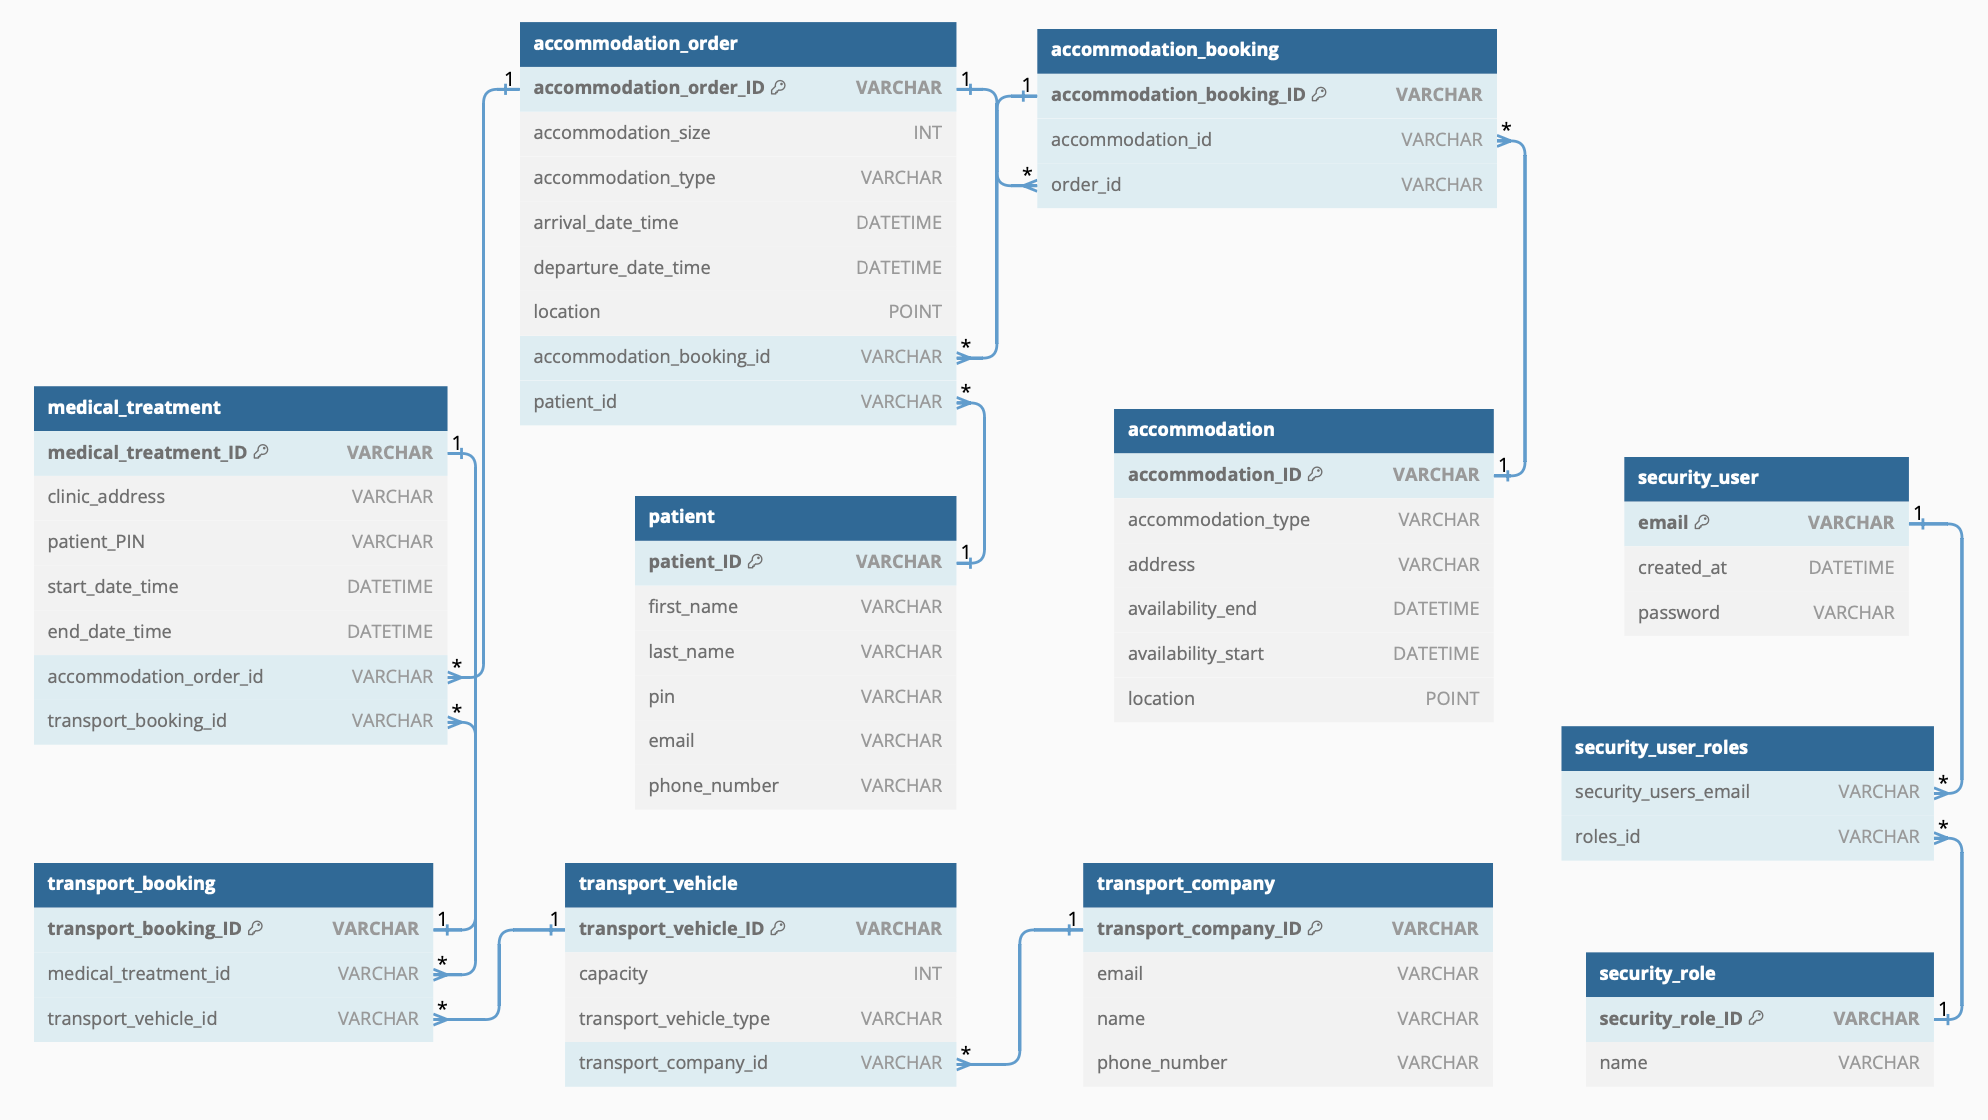
\includegraphics[scale=0.42]{slike/dijagram_baze_v2.png} %veličina slike u odnosu na originalnu datoteku i pozicija slike
					\centering
					\caption{ER Dijagram baze podataka}
					\label{fig:dijagram_baze_podataka}
				\end{figure}
			
			\eject
			
			
		\section{Dijagram razreda}
		
			Na slikama \ref{fig:arhitektura_controller_class_diagram}  do \ref{fig:arhitektura_model_class_diagram}  prikazani su ključni elementi backend dijela arhitekture DentAll aplikacije. 
			
			Prva slika \ref{fig:arhitektura_controller_class_diagram}  prikazuje dijagram razreda Controllera, prikazujući sve Controller razrede u aplikaciji.  Sljedeći veliki element arhitekture backenda su Service sučelja i pripadajući ServiceImpl razredi prikazani na \ref{fig:arhitektura_service_class_diagram}. Slika \ref{fig:arhitektura_dto_class_diagram} fokusira se na dijagram razreda s DTO razredima koje služe za prijenos podataka između Controllera i Modela. Svaka DTO klasa odgovara određenom razredu iz Modela, osiguravajući učinkovit prijenos podataka unutar aplikacije. Na slici \ref{fig:arhitektura_requests_class_diagram} nalaze se Requests razredi koje predstavljaju zahtjeve od klijenta prema Controller razredima. Ovi razredi sadrže sve potrebne informacije za izvođenje funkcionalnosti poput CREATE i UPDATE. Obuhvaćajući sve domain razrede iz modela DentAll aplikacije, dijagram razreda sa slike  \ref{fig:arhitektura_model_class_diagram} prikazuje relacije i međusobnu povezanost između razreda unutar modela. Svaki segment dokumentacije dijagrama razreda osmišljen je da naglasi važnost svakog dijela arhitekture u dizajnu i implementaciji sustava.
			
						
			\begin{figure}[H]
				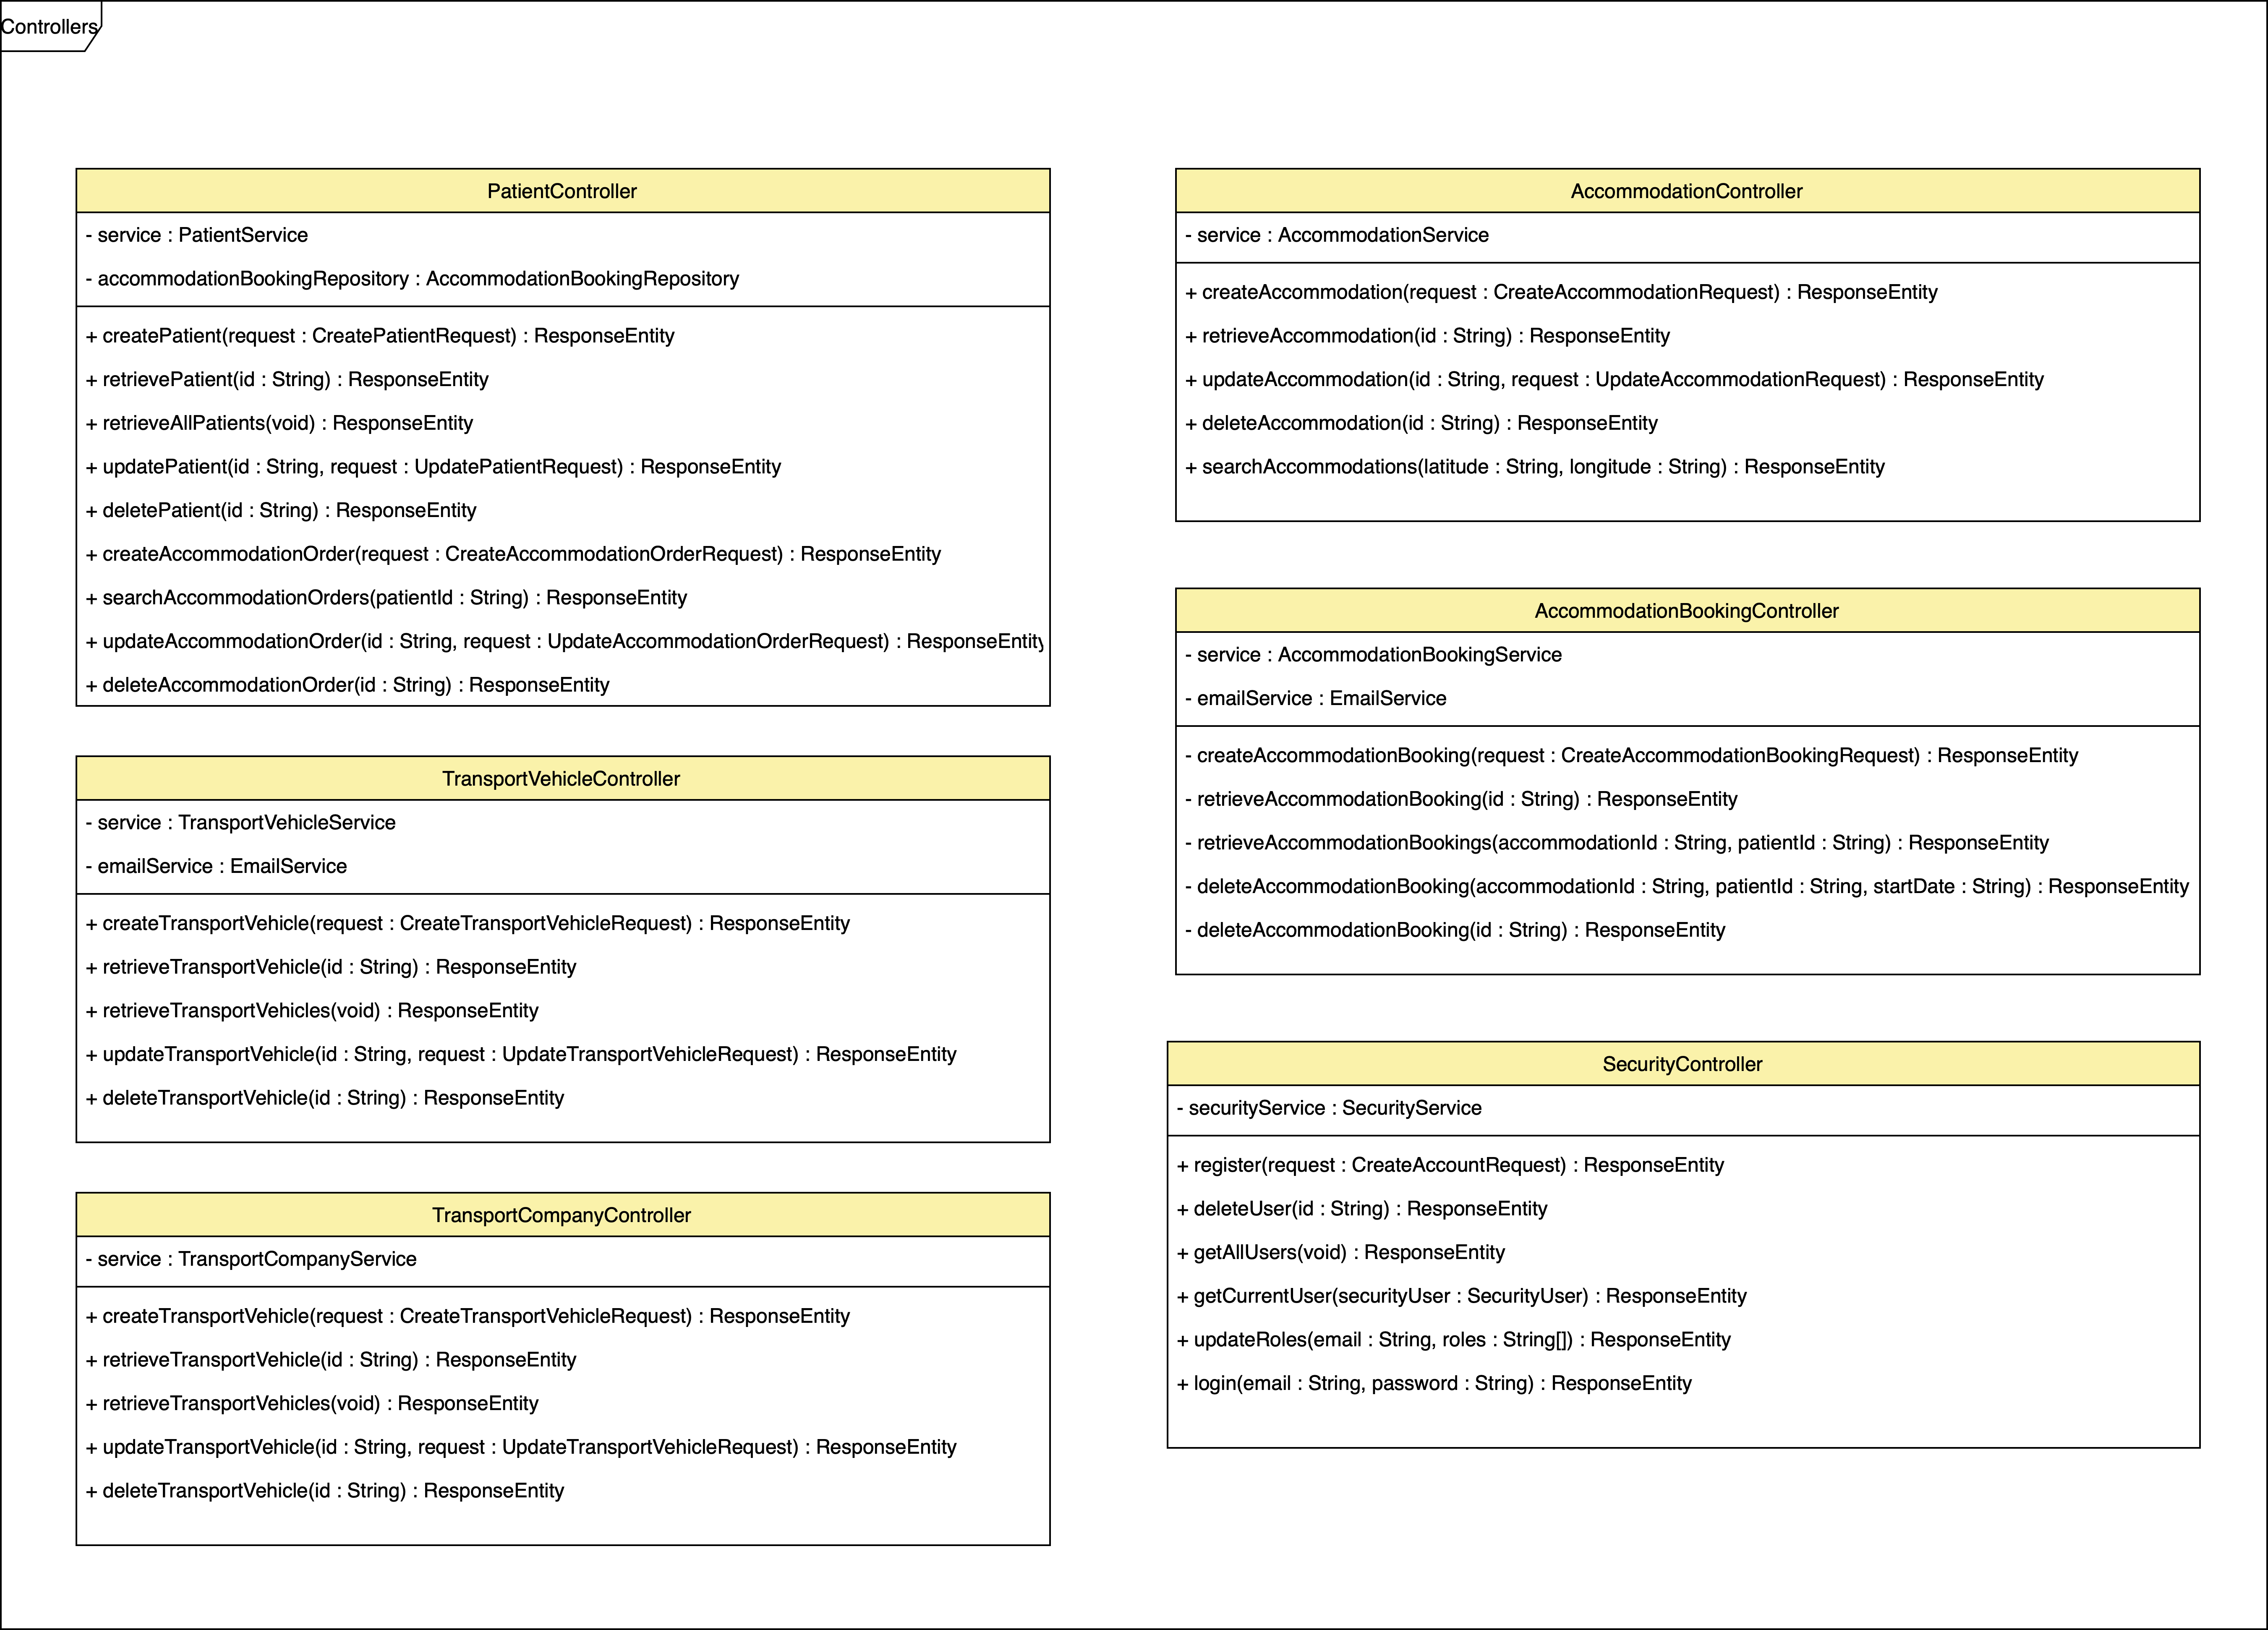
\includegraphics[scale=0.07]{slike/arhitektura_controller_class_diagram_v2.png} %veličina slike u odnosu na originalnu datoteku i pozicija slike
				\centering
				\caption{Dijagram razreda - dio Controllers}
				\label{fig:arhitektura_controller_class_diagram}
			\end{figure}
			
			Kontroleri su poveznica između korisnika i aplikacije, odgovorni za upravljanje okom HTTP zahtjeva i odgovora. Svaki Controller razred u DentAll aplikaciji povezan je s određenim Service sučeljem koji omogućuje obradu poslovne logike. PatientController upravlja pacijentima i sadrži metode poput createPatient i deletePatient, koje prate RESTful princip za CRUD operacije. TransportVehicleController i TransportCompanyController omogućavaju upravljanje vozilima i tvrtkama za transport, s metodama kao što su createTransportVehicle i updateTransportCompany. AccommodationController i AccommodationBookingController služe za upravljanje smještajem te njegovu rezervaciju kroz booking. SecurityController upravlja autentifikacijom i autorizacijom, s metodama poput register i login.
			
			\begin{figure}[H]
				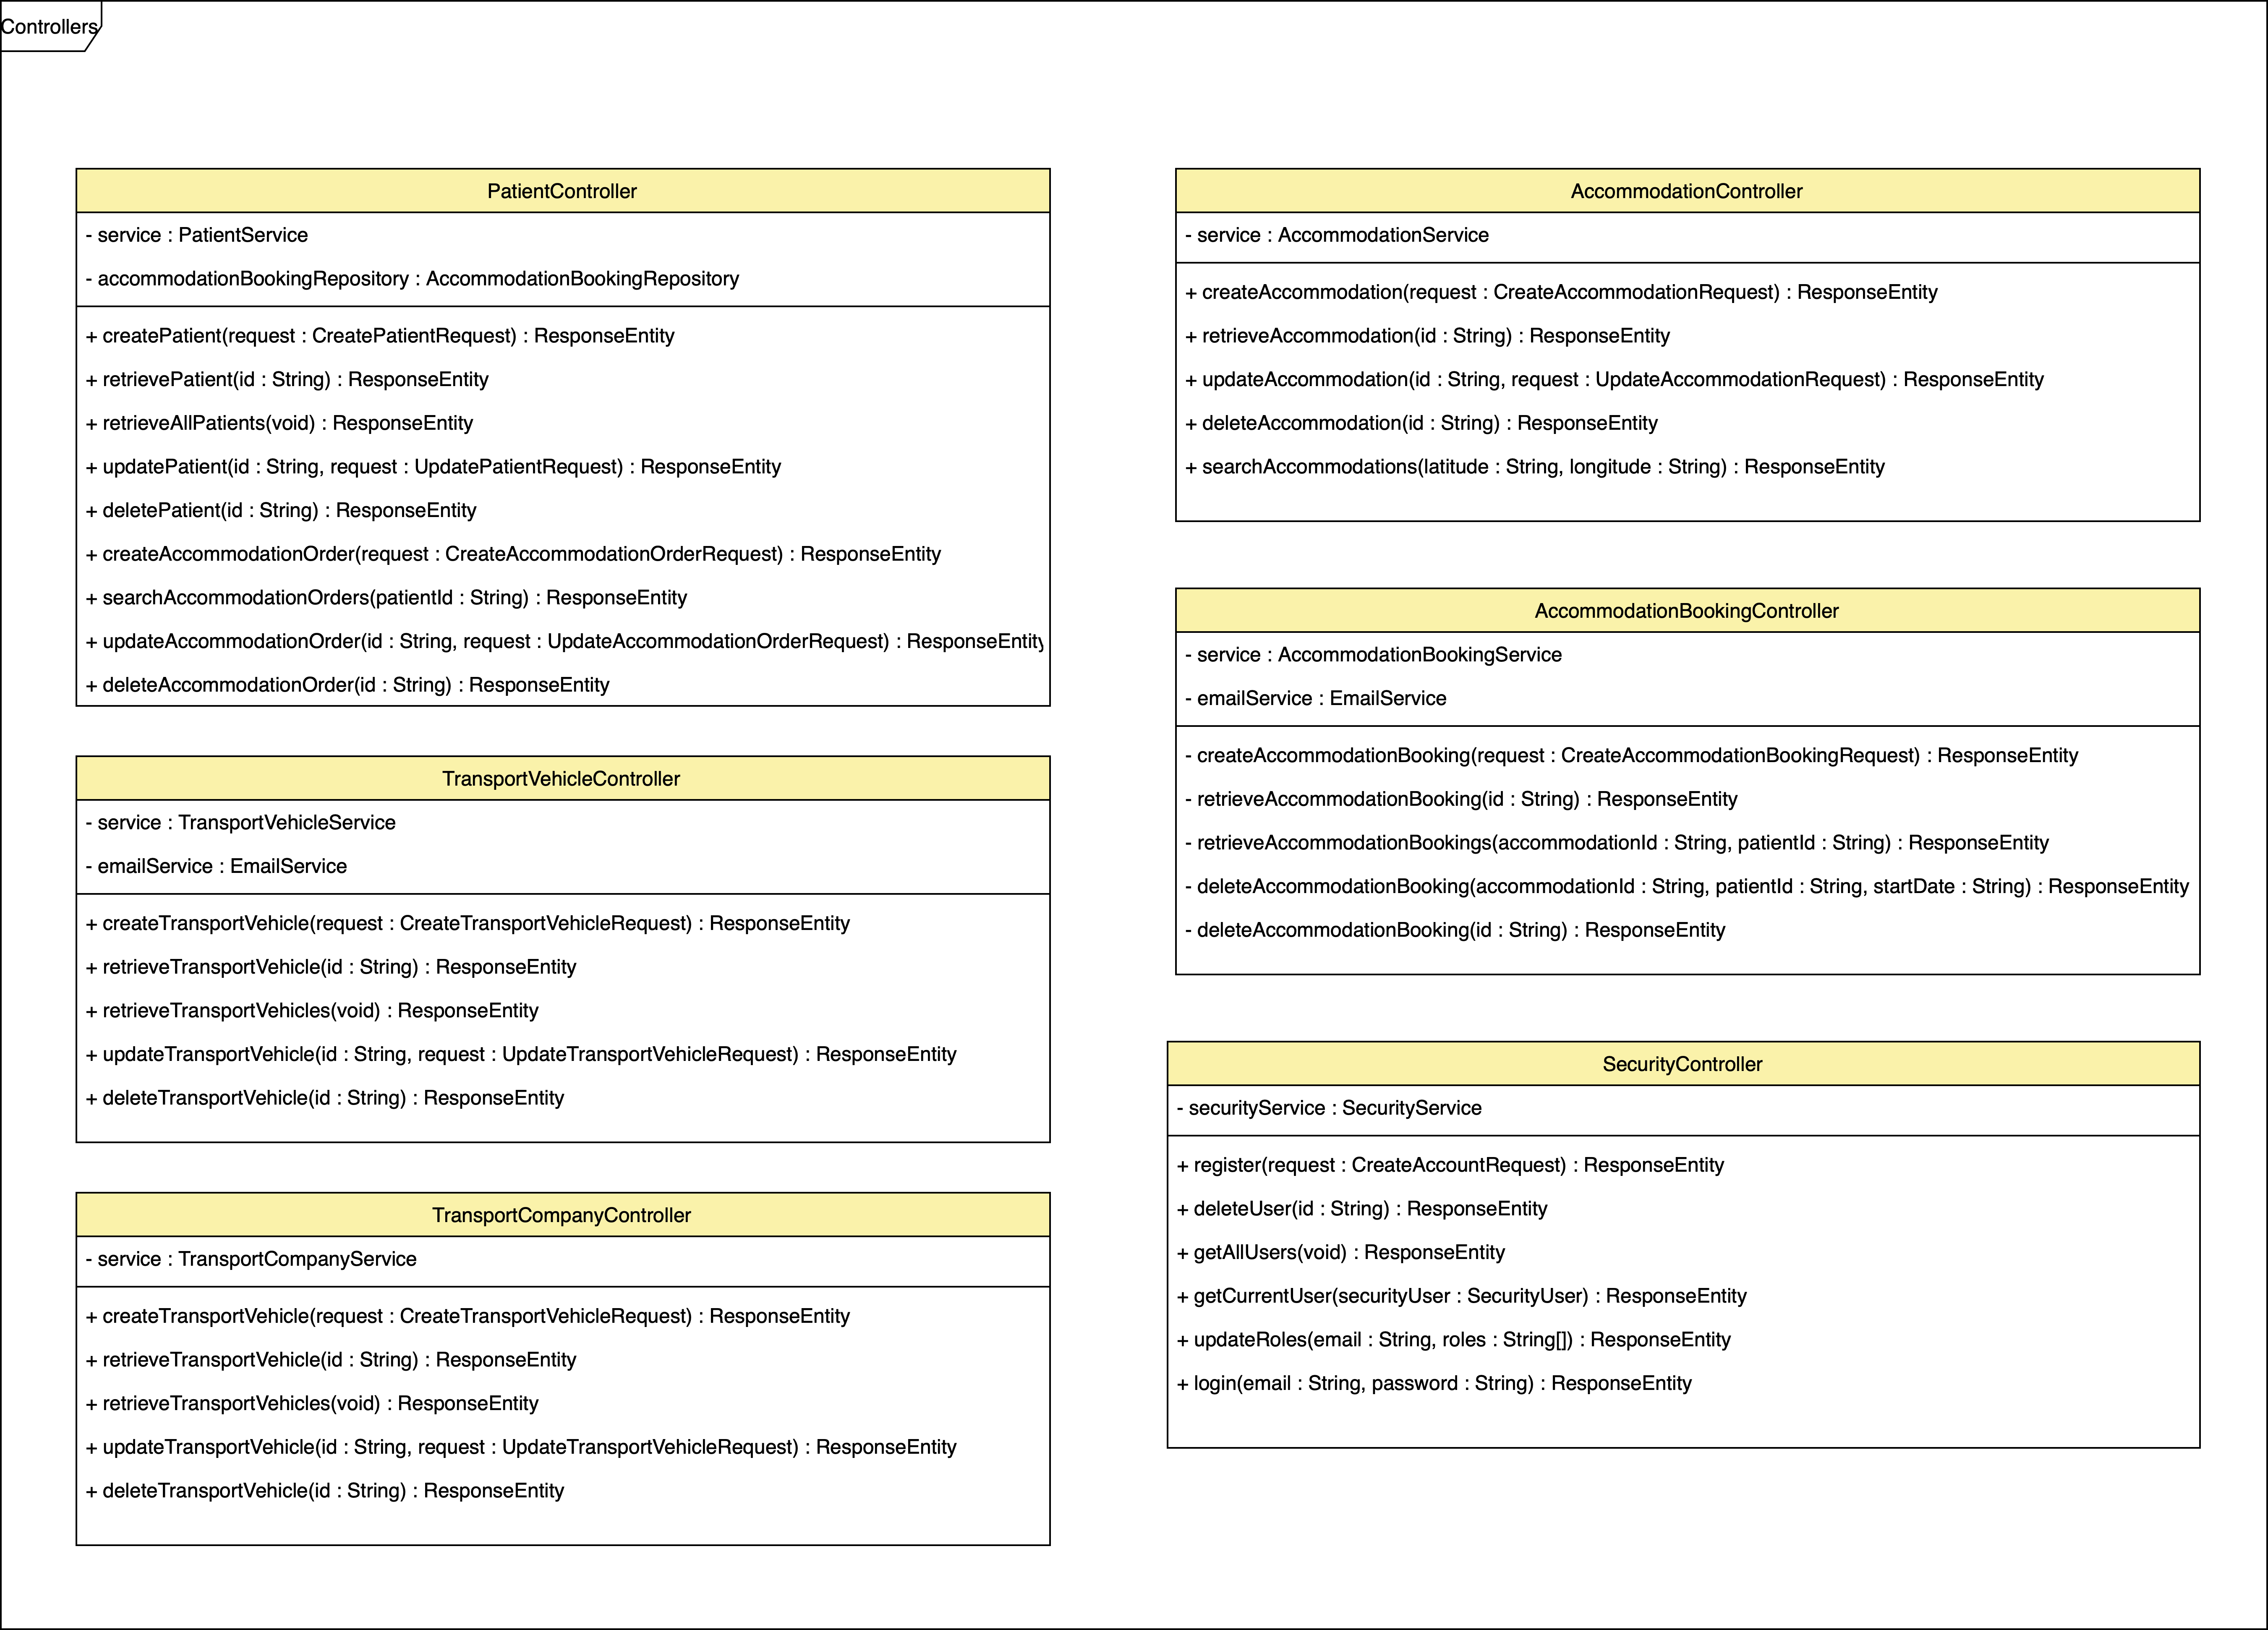
\includegraphics[scale=0.07]{slike/arhitektura_controller_class_diagram_v2.png} %veličina slike u odnosu na originalnu datoteku i pozicija slike
				\centering
				\caption{Dijagram razreda - dio Service}
				\label{fig:arhitektura_service_class_diagram}
			\end{figure}
			
			*Insert opis za Service i ServiceImpl*
			
			\begin{figure}[H]
				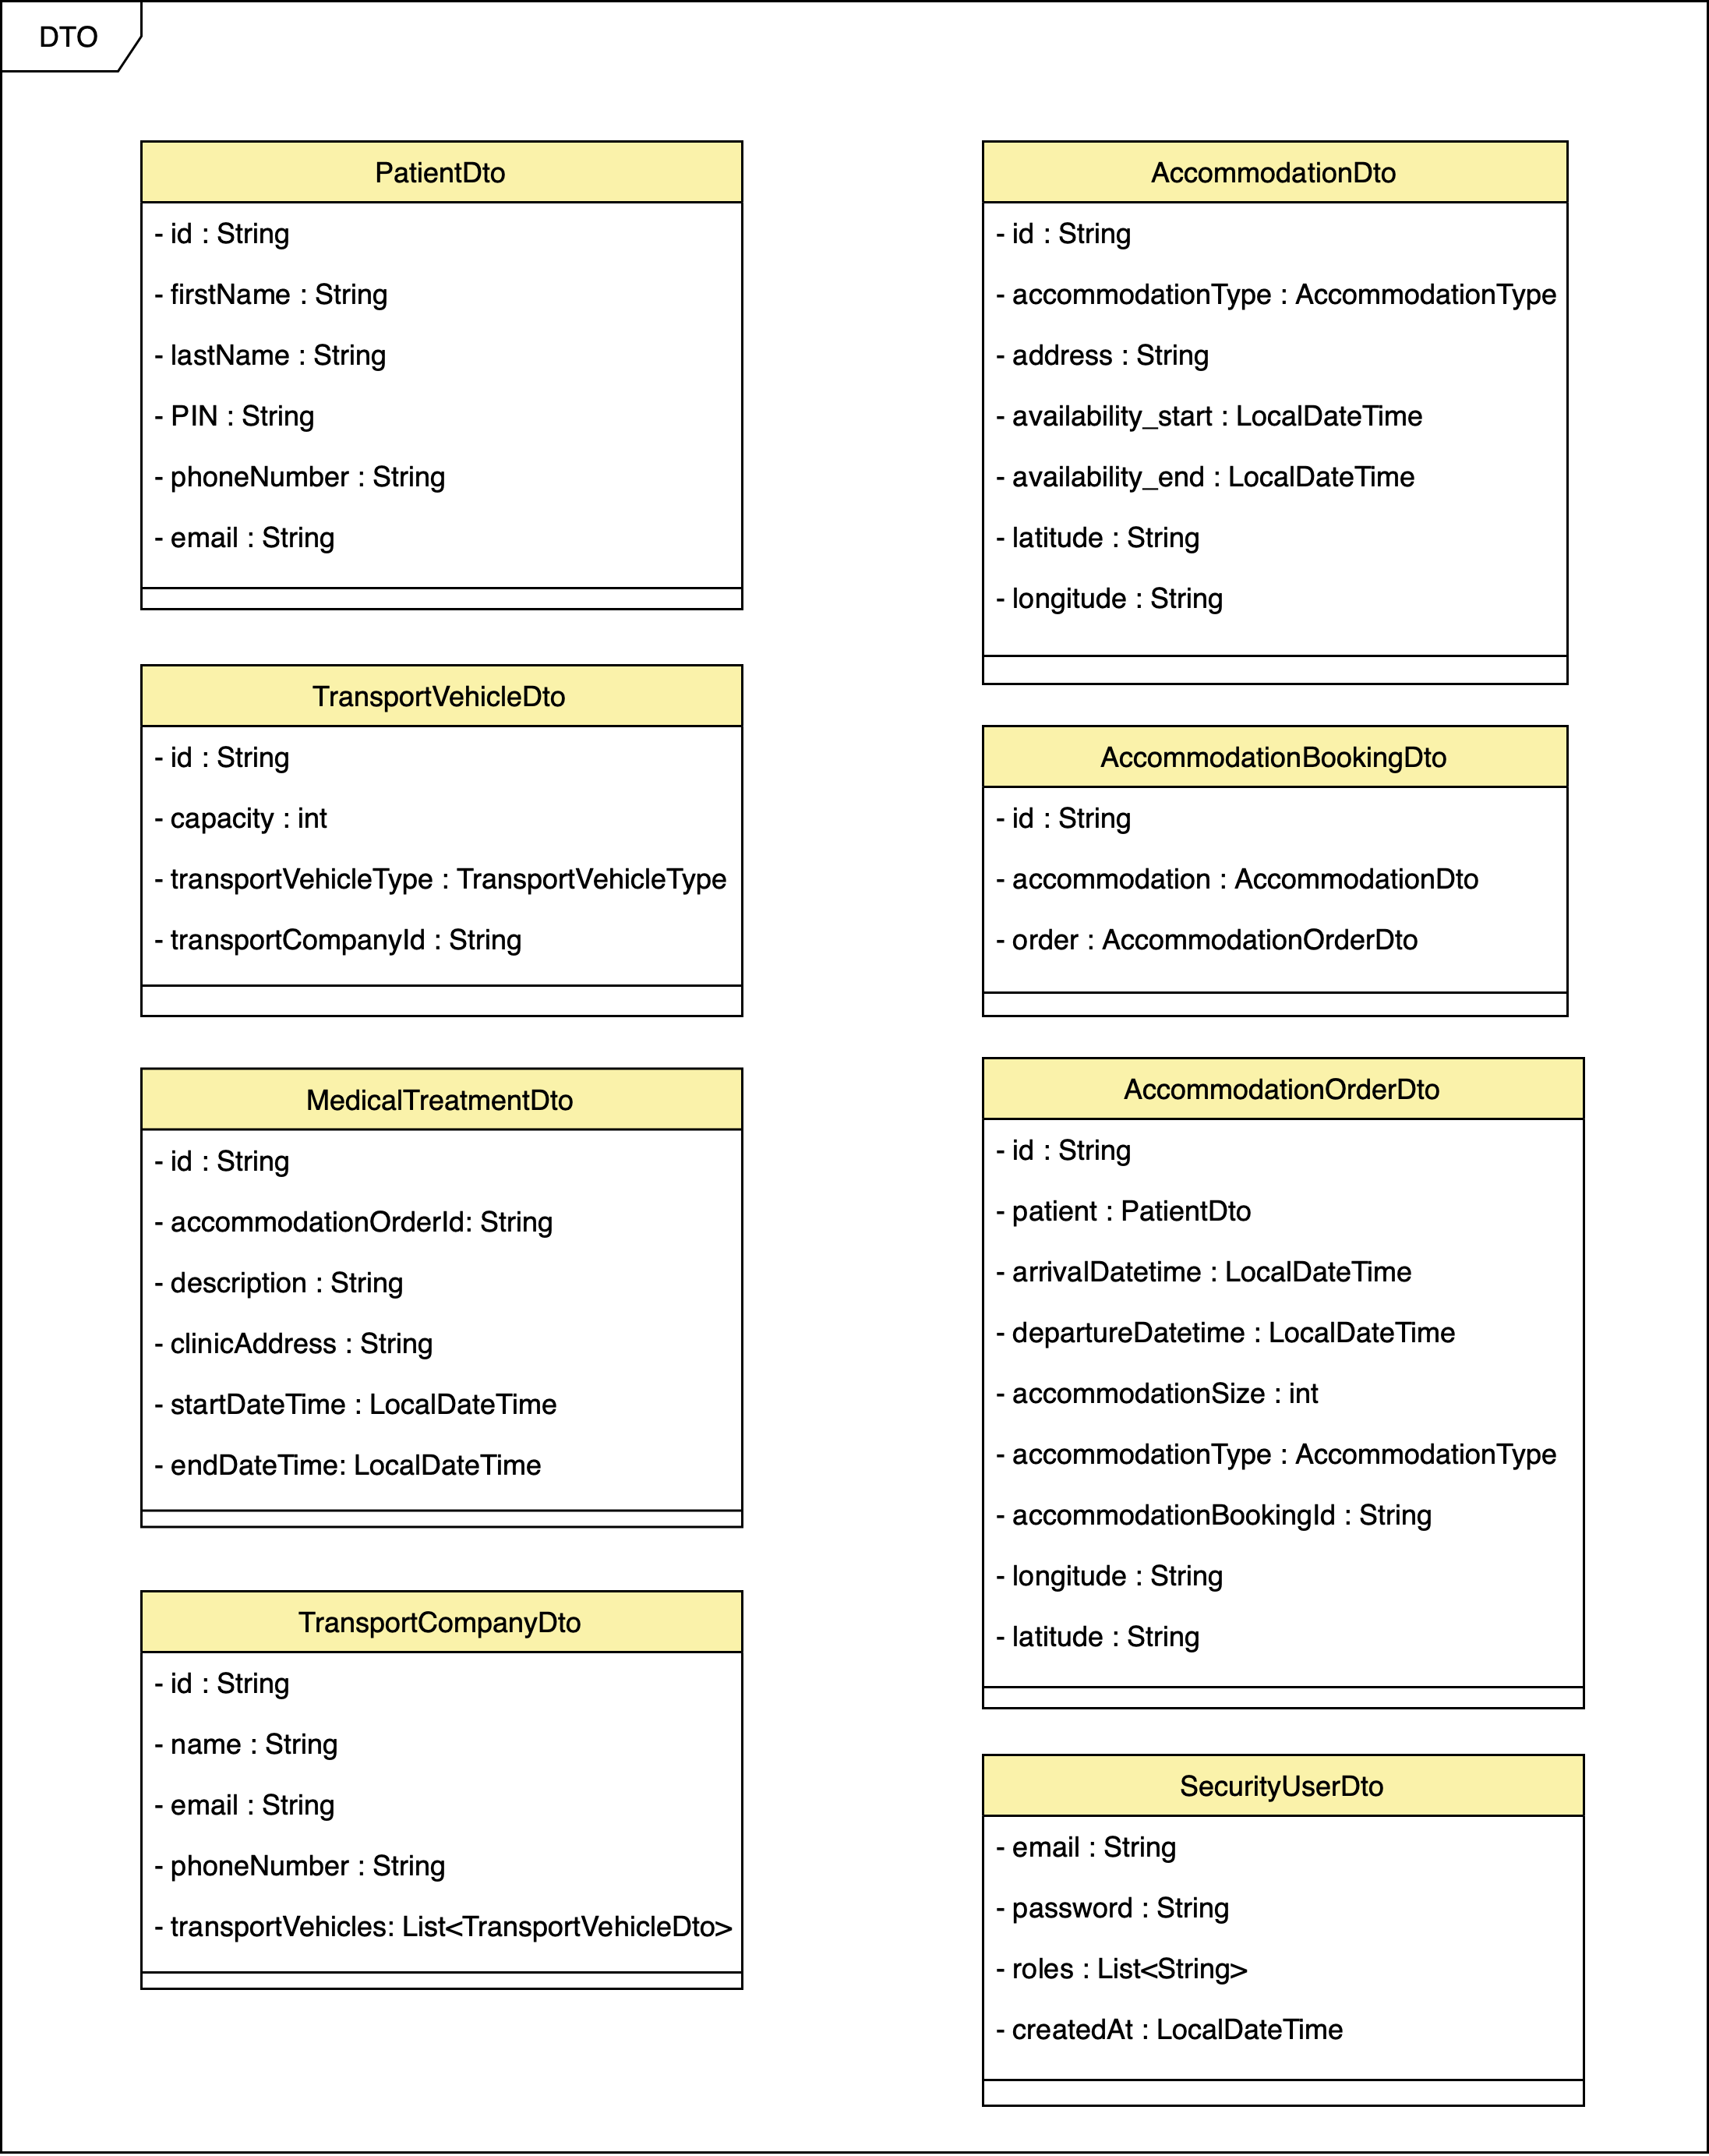
\includegraphics[scale=0.12]{slike/arhitektura_dto_class_diagram_v2.png} %veličina slike u odnosu na originalnu datoteku i pozicija slike
				\centering
				\caption{Dijagram razreda - dio DTO}
				\label{fig:arhitektura_dto_class_diagram}
			\end{figure}
			
			DTO razredi su ključni za učinkovit i siguran prijenos podataka između slojeva aplikacije. DTO omogućuje da se modeli ne izlažu direktno klijentima, što smanjuje rizik od manipulacije podataka. Svaki DTO sadrži atribute koji se mapiraju na entitet modela, uz potrebne gettere i settere za pristup i modifikaciju podataka.
			
			\begin{figure}[H]
				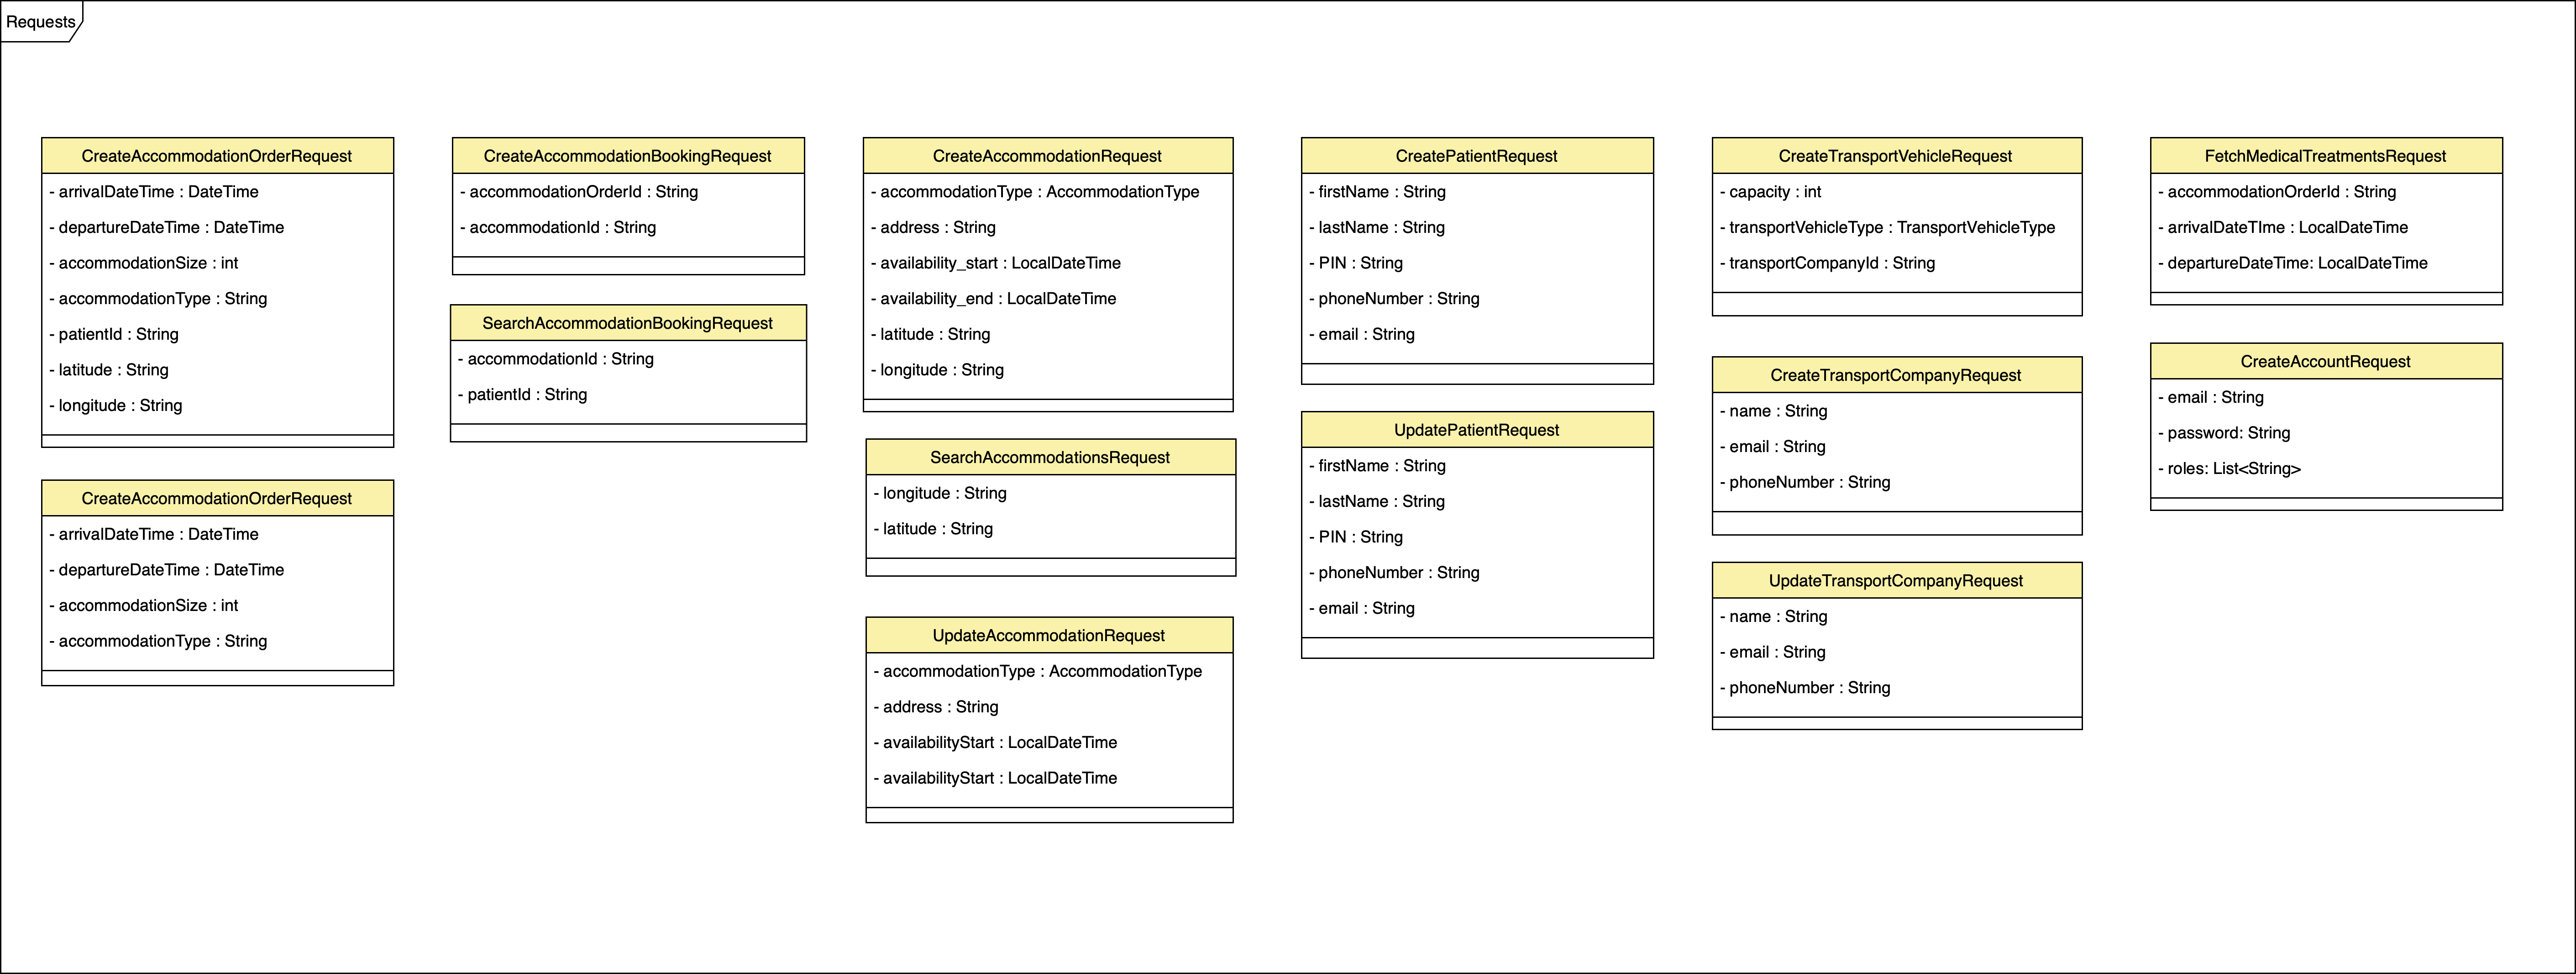
\includegraphics[scale=0.08]{slike/arhitektura_requests_class_diagram_v2.png} %veličina slike u odnosu na originalnu datoteku i pozicija slike
				\centering
				\caption{Dijagram razreda - dio Requests}
				\label{fig:arhitektura_requests_class_diagram}
			\end{figure}
			
			Request razredi su specijalizirani razredi koji sadrže sve potrebne informacije za obradu zahtjeva. Oni olakšavaju validaciju ulaznih podataka i smanjuju složenost Controller razreda.
			
			\begin{figure}[H]
				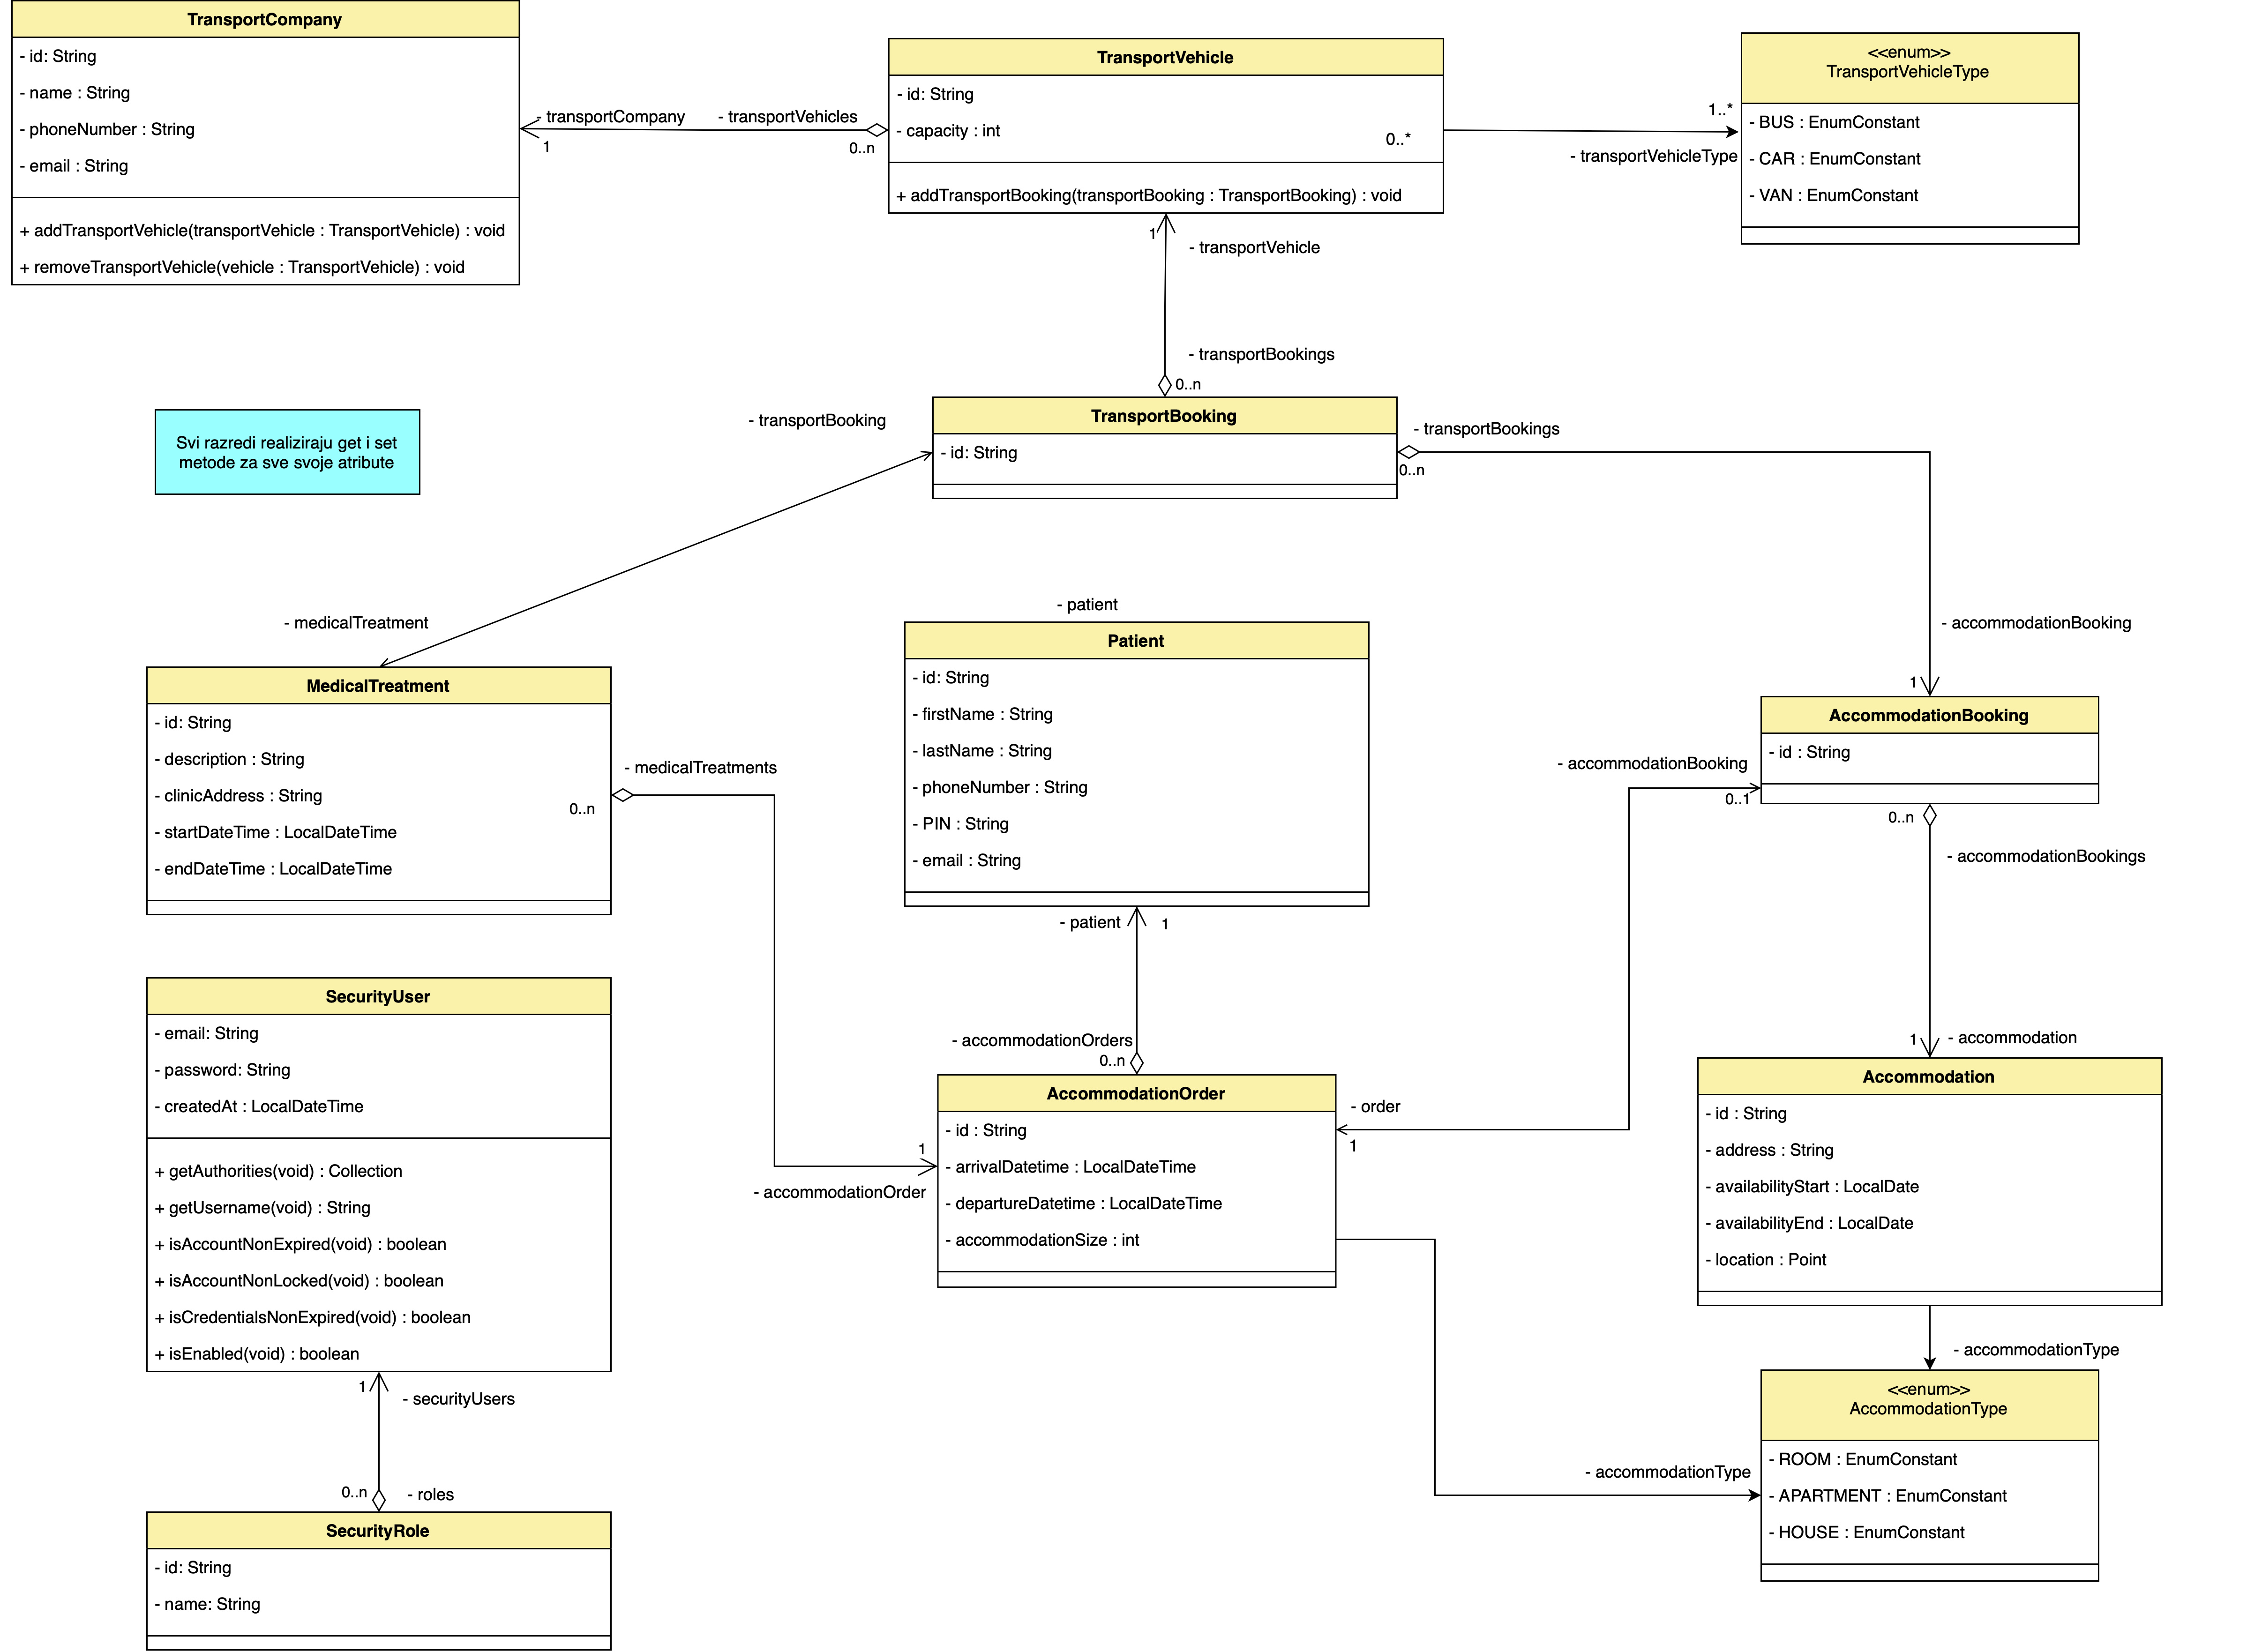
\includegraphics[scale=0.08]{slike/arhitektura_model_class_diagram_v2.png} %veličina slike u odnosu na originalnu datoteku i pozicija slike
				\centering
				\caption{Dijagram razreda - dio Model}
				\label{fig:arhitektura_model_class_diagram}
			\end{figure}
			
			 Domain modeli su osnovni razred nad kojim se obrađuje sve u aplikaciji.  Patient, TransportVehicle, Accommodation, i AccommodationOrder su osnovni entiteti koji se međusobno povezuju. Odnosi između entiteta su jasno definirani s odgovarajućim vezama (npr. jedan pacijent može imati više medicinskih tretmana). SecurityUser i SecurityRole modeliraju sigurnosni aspekt aplikacije, omogućavajući upravljanje pristupom i autorizacijom. 
			
			
			\eject
		
		\section{Dijagram stanja}
			
			
			\textbf{\textit{dio 2. revizije}}\\
			
			\textit{Potrebno je priložiti dijagram stanja i opisati ga. Dovoljan je jedan dijagram stanja koji prikazuje \textbf{značajan dio funkcionalnosti} sustava. Na primjer, stanja korisničkog sučelja i tijek korištenja neke ključne funkcionalnosti jesu značajan dio sustava, a registracija i prijava nisu. }
			
			
			\eject 
		
		\section{Dijagram aktivnosti}
			
			Dijagram aktivnosti primjenjuje se za opis modela toka upravljanja ili toka podataka. Ne upotrebljava se za modeliranje događajima poticanog ponašanja. 
			Na dijagramu aktivnosti \ref{fig:dijagram-aktivnosti} prikazan je proces kreiranja zahtjeva za smještaj, dohvaćanja medicinskih termina te rezervacije vozila za termine. Korisnički administrator unosi zahtjeve za smještaj u sustav se prijavi u sustav. U sustavu se svakih 10 sekundi provjerava postoji li zahtjev za smještaj ( dolazak pacijenta ) koji još nema medicinske termine. Za sve koji nemaju medicinske termine zove se Aplikacija za medicinske usluge ( external API ) koji vraća za sve zahtjeve nasumično 0, 1, 2 ili 3 medicinska termina unutar zadanog vremena dolaska i odlaska pacijenta definiranih u zahtjevu. Također, svakih 10 sekundi se provjerava i postoje li i medicinski termini koji još nemaju rezervirano vozilo za prijevoz. Za sve koji nemaju dodjeljuje se vozilo, ako postoji u terminu medicinske usluge, s uvjetom da pacijent već ima rezerviran smještaj.
			
			\begin{figure}[H]
				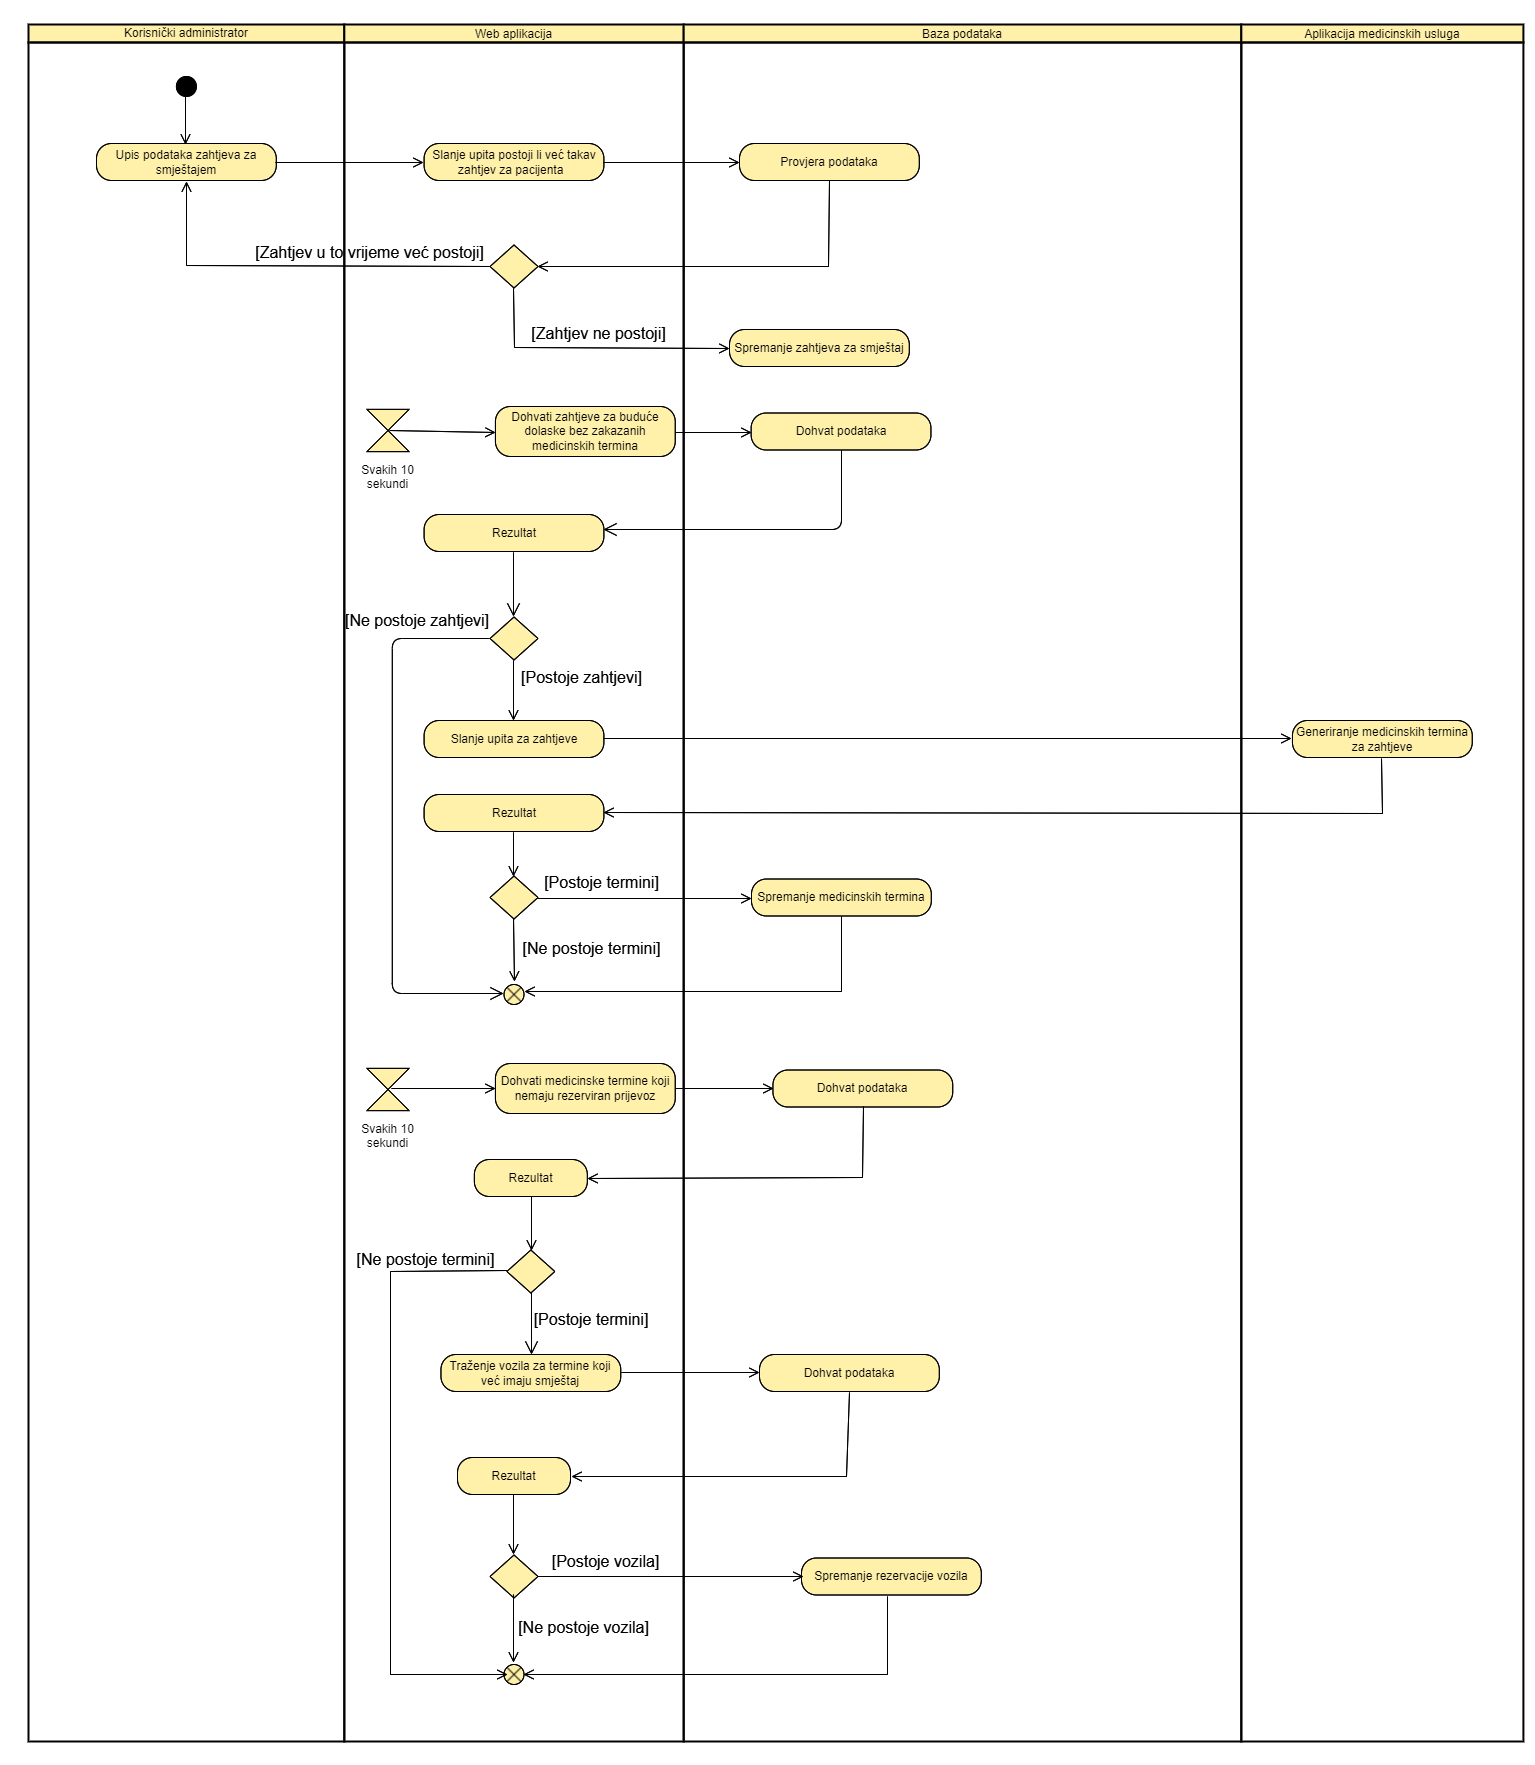
\includegraphics[width=\textwidth]{slike/activityDiagram.png}
				\centering
				\caption{Dijagram aktivnosti}
				\label{fig:dijagram-aktivnosti}
			\end{figure}
			
			\eject
		\section{Dijagram komponenti}
			
			Na donjoj slici 4.9 prikazan je dijagram komponenti koji
			vizualno prikazuje ovisnost komponenti. Aplikacija DentAll
			sastoji se od tri komponente: frontend, backend i Medical Service. 
			Komponenta frontenda napravljena je korištenjem biblioteke React, a komponenta
			backenda izgrađena je pomoću Java Spring Boota. Na slici je označeno da 
			korisnik preko web preglednika pristupa aplikaciji, komponente frontend 
			i backend međusobno razmjenjuju podatke preko REST\_API-ja, baza podataka
			komunicira sa backendom preko SQL upita, a komponenta Medical Service
			komunicira sa backendom putem REST\_API-ja.
			
			\begin{figure}[H]
				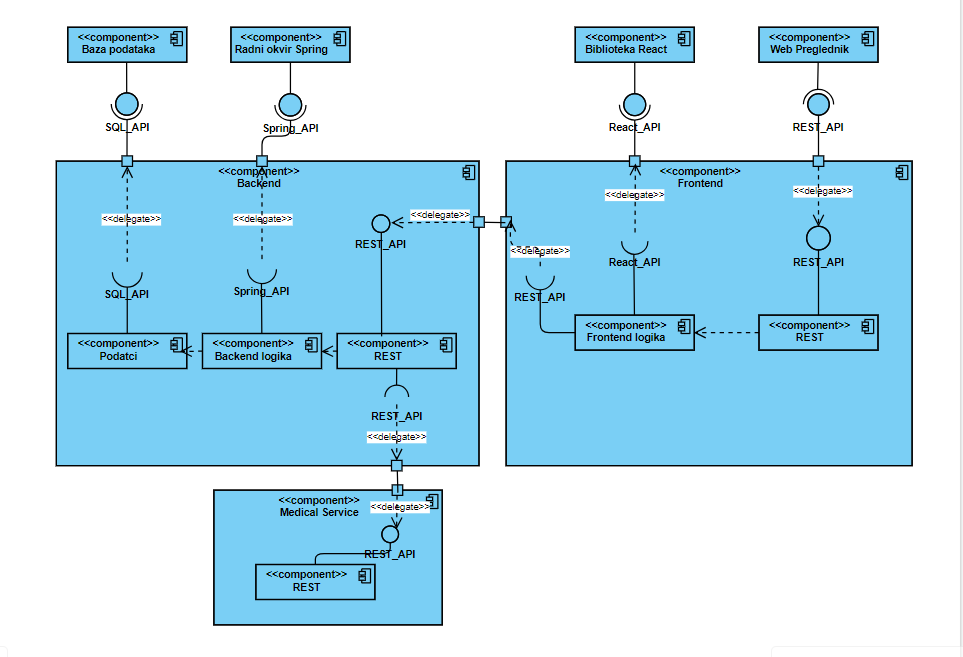
\includegraphics[width=\textwidth]{slike/dijagram_komponenti.png}
				\centering
				\caption{Dijagram aktivnosti}
				\label{fig:dijagram-komponenti}
			\end{figure}